%%%%%%%%%%%%%%% Start of Title Page %%%%%%%%%%%
\begin{titlepage}
\begin{center}
\textit{Heaven's Light is Our Guide}
\\[0.5cm]
\textbf{\Large Rajshahi University of Engineering \& Technology}
\\[0.3cm] 
\textbf{\large Department of Electronics \& Telecommunication Engineering}
\\[0.2cm]
\begin{figure}[!htbp]
    \centering
    
\includegraphics[scale=0.3]{Figures/logo_ruet}
    \label{fig:RUET logo}
\end{figure}
\textbf{\Large EEE1254: Sessional Based on EEE1253 }
\\[0.5cm]
\myrule[1pt][5pt]

%%%%%%%%%%%%%%%%%%%%%%%%%%%%%%%%%%%%%%%%%%%%%%%
%%%%%%%%%%%%%%% STUDENT'S INFO %%%%%%%%%%%%%%%%
%%%%%%%%%%%%%%%%%%%%%%%%%%%%%%%%%%%%%%%%%%%%%%%

\textbf{\Large  Experiment No. \ref{exp2}}
\\[.25cm]
\textbf{\large No Load Magnetization of a Separately Excited DC Generator}
\\ 
\myrule[1pt][5pt] 
\begin{minipage}{0.4\textwidth}
\vspace{0.5cm}
\begin{flushleft} 
\emph{\textbf{\large Submitted by:}}
\\
Antu Roy Chowdhury \\
Roll: 2004050 \\
Session: 2020-21
\end{flushleft}
\end{minipage}
~
\begin{minipage}{0.4\textwidth}
\vspace{0.5cm}
\begin{flushright} 
\emph{\textbf{\large Submitted to:}} 
\\
A. S. M. Badrudduza
\\
Assistant Professor
\\
Dept. of ETE, RUET
\\
\end{flushright}
\end{minipage}\\[0.7cm]
\makeatother

\textbf{Date of Experiment : 27/09/2022}\\
\textbf{Date of Submission : 11/10/2022}\\[1cm]

%************** End of Student's Info *********


\vfill
%%%%%%%%%%%%%%% TEACHER SECTION %%%%%%%%%%%%%%%
\hrulefill
\vspace{-5mm}
\begin{multicols}{3}
\begin{itemize} [labelindent=3em,labelsep=0.5cm,leftmargin=*,noitemsep]
        \item[] \textbf{\underline{Report}}
        \item[$\square$] Excellent
        \item[$\square$] Very Good
        \item[$\square$] Good
        \item[$\square$] Average
        \item[$\square$] Poor
\end{itemize}
\columnbreak
\textbf{(Teacher's Section)}
\\[1.5cm]
--------------------------------
\\
Signature
\columnbreak
\begin{itemize}
[labelindent=6em,labelsep=0.5cm,leftmargin=*,noitemsep]
        \item[] \textbf{\underline{Viva}}
        \item[$\square$] Excellent
        \item[$\square$] Very Good
        \item[$\square$] Good
        \item[$\square$] Average
        \item[$\square$] Poor
\end{itemize}
\end{multicols}
\end{center}
\end{titlepage}
\newpage
%************** End of Teacher Section ********
%************** End of Title Page *************


%%%%%%%%%%%%%%% Exp. Positioning %%%%%%%%%%%%%%
\titleformat{\chapter}[display]
  {\normalfont\large\bfseries}{\chaptertitlename\ \thechapter}{0pt}{\large}
\titlespacing*{\chapter}{0pt}{-15pt}{10pt}
% \addcontentsline{lof}{chapter}{\protect\numberline{ \ref{exp1}}}
% \addcontentsline{lot}{chapter}{\protect\numberline{ \ref{exp1}}}
%************** End of Exp. Positioning *******


%%%%%%%%%%%%%%%%%%%%%%%%%%%%%%%%%%%%%%%%%%%%%%%
%%%%%%%%%%%%%%% Student's Part %%%%%%%%%%%%%%%%
%%%%%%%%%%%%%%% Start of Report %%%%%%%%%%%%%%%
%%%%%%%%%%%%%%%%%%%%%%%%%%%%%%%%%%%%%%%%%%%%%%%


%**********************************************
\chapter{No Load Magnetization of a Separately Excited DC Generator}
\label{exp2}


%**********************************************
\section{Objectives}
The main objectives of this experiment are
\begin{itemize}
    \item To understand the characteristics of a separately excited DC generator.
    \item To understand the no load magnetization curve of a separately excited DC generator
    \item To learn how the the induced voltage can be controlled with the help of the changing resistor.
    \item To be able to plot the no load magnetization curve.
\end{itemize}


%**********************************************
\section{Theory}
Voltage can be gained from a DC generator if the changing of flux in the coil and the speed of the armature of the DC generator can be increased. So the multiplication of the lines of the flux and the speed of the armature is proportional to the voltage induced in the generator. As shown in Figure \ref{fig:figg1} .
\FloatBarrier
\begin{figure}[hbt!]
\vspace{00mm}
    \centerline{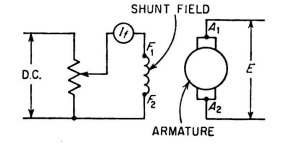
\includegraphics[width=0.6\textwidth]{Figures/Exp02/machine Lab 2 .jpeg}}
    \vspace{0mm}
    \caption{Circuit to obtain no lead saturation curve.}
    \label{fig:figg1}
\end{figure}
\newpage
So the formula of the voltage produced in a DC generator can be written as,
\begin{align}
\nonumber
E \infty S\phi
\\
=> E = KS\phi
\end{align}
where,
\begin{align}
    \nonumber
    K=\frac{Z}{a}\times P\times \frac{1}{60}\times10^{-8}
    \\\nonumber
    \phi = lines of flux per pole 
    \\\nonumber
    S = speed of the armature
\end{align}
Residual magnetism is a phenomena which determines the amount of magnetization in a circuit which is remained after the removal of the external magnetic field from the circuit. Due to this phenomena when the circuit current is zero, yet a very small amount of voltage is found on the generator. This indicates the point 1 is figure \ref{fig:figg2} . 

\begin{figure}[hbt!]
\vspace{00mm}
    \centerline{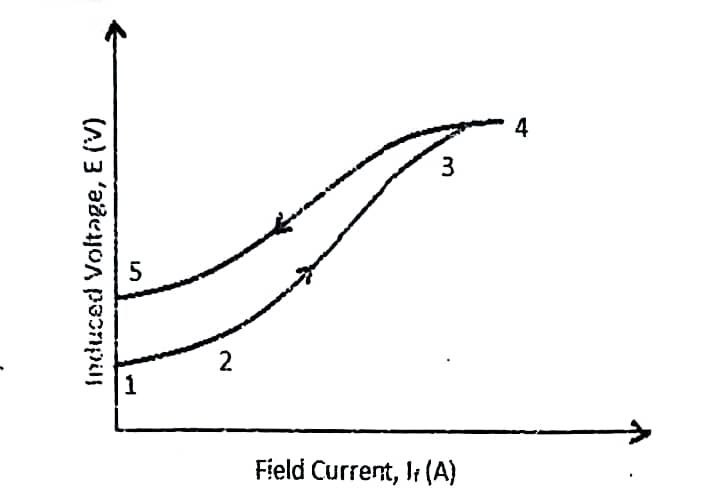
\includegraphics[width=0.6\textwidth]{Figures/Exp02/Lab 1 residual magnetization.jpeg}}
    \vspace{0mm}
    \caption{No load saturation curve.}
    \label{fig:figg1}
\end{figure}
If the current increases then the voltage will also increase. From point 2 to point 3  , the relation between the current and the induced voltage is almost proportional for which it gives a straight line from point 2 to 3. Point 3 is called the knee point because beyond this point, no matter how much the current is increased, the voltage does not increase proportionally. From point 3 to 4, this phenomena continues and it finally reaches the saturation point of the curve in point 4 of the fig \ref{fig:figg2} . Point 3 to 4 is called the above the knee part of the graph. After the saturation point is gained if the current is decreased then the graph will reach at point 5. But the path of the curve will not be the same while decreasing the current. That will create a hysteresis loop.


%**********************************************
\section{Required Apparatus}
\begin{enumerate}
\item Generator (250 V, 18 A). 
\item Prime mover (Induction motor 1420 rpm/synchronous motor -1 500 rpm). 
\item  Tachometer. 
\item Voltmeter (0-450 V). 
\item Ammeter (0-2 A).
\end{enumerate}




%**********************************************
\section{Circuit Diagram}
\begin{figure}[hbt!]
\vspace{00mm}
    \centerline{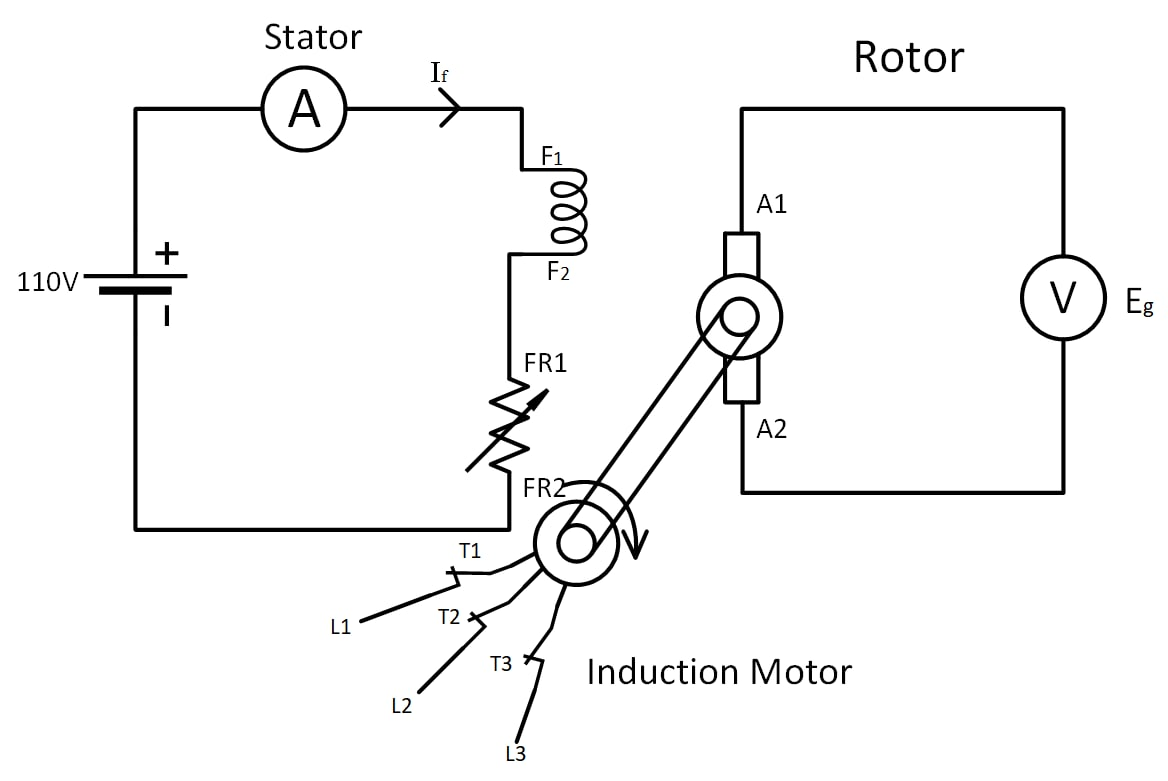
\includegraphics[width=1\textwidth]{Figures/Exp02/circuit diagram.jpeg}}
    \vspace{0mm}
    \caption{Circuit diagram for separated excited dc generator}
    \label{fig:figg2}
\end{figure}


%**********************************************
\section{Procedure}


%**********************************************
\subsection{Increasing of the current}
\begin{itemize}

    \item Supply voltage was set to 110 V.
    
    \item An ammeter and a voltmeter was connected with the circuit and all the other connection was completed as shown in the circuit diagram.
    
    \item The switch of the induction motor was turned on, the rotation was checked. If the rotation was not found accurately then any two connections between $T_1, T_2, T_3,$ was interchanged to fix the rotation. 
    
    \item The speed of the motor was maintained at a fixed speed with the help of tachometer and the speed was measured in RPM. 
    
    \item The value of current in the generator coil was increased by varying the rheostat . The value of resistance was decreased so that the current increased. Then the changing of the voltage across the rotor was measured.
    
    \item Finally, the values of the current and the voltage were plotted on graph paper.
    
\end{itemize}



%**********************************************
\subsection{Decreasing of the current}
\begin{itemize}

    \item After reaching the saturated voltage, the current was reduced by increasing the value of resistor and when the current reached 0 ampere again then the residual voltage was calculated.
    .
    \item Finally, the values of the current and the voltage were plotted on graph paper.
    
\end{itemize}



%**********************************************
\newpage
\section{Data Table}
\begin{table}[hbt!]
\centering
\caption{No load magnetization of a separately excited DC generator}
\label{tab1}
% Please add the following required packages to your document preamble:
% \usepackage{multirow}

\begin{tabular}{|c|c|cc|cc|c|}
\hline
\multirow{2}{*}{\begin{tabular}[c]{@{}c@{}}Obs.\\ no.\end{tabular}} &
  \multirow{2}{*}{\begin{tabular}[c]{@{}c@{}}Field\\ DC \\ Supply\\ (V)\end{tabular}} &
  \multicolumn{2}{c|}{Increasing Current} &
  \multicolumn{2}{c|}{Decreasing Current} &
  \multirow{2}{*}{\begin{tabular}[c]{@{}c@{}}Speed\\ (rpm)\end{tabular}} \\ \cline{3-6}
 &
   &
  \multicolumn{1}{c|}{\begin{tabular}[c]{@{}c@{}}Field \\ Current,\\ If(A)\end{tabular}} &
  \begin{tabular}[c]{@{}c@{}}Induced \\ Voltage,\\ Eg(V)\end{tabular} &
  \multicolumn{1}{c|}{\begin{tabular}[c]{@{}c@{}}Field \\ Current,\\ If(A)\end{tabular}} &
  \begin{tabular}[c]{@{}c@{}}Induced\\ Voltage,\\ Eg(V)\end{tabular} &
   \\ \hline
1. & \multirow{8}{*}{110V} & \multicolumn{1}{c|}{0}    & 5.15 & \multicolumn{1}{c|}{0.31} & 172   & \multirow{8}{*}{1472} \\ \cline{1-1} \cline{3-6}
2. &                       & \multicolumn{1}{c|}{0.15} & 100  & \multicolumn{1}{c|}{0.3}  & 170.4 &                       \\ \cline{1-1} \cline{3-6}
3. &                       & \multicolumn{1}{c|}{0.2}  & 118  & \multicolumn{1}{c|}{0.26} & 156   &                       \\ \cline{1-1} \cline{3-6}
4. &                       & \multicolumn{1}{c|}{0.22} & 129  & \multicolumn{1}{c|}{0.24} & 148   &                       \\ \cline{1-1} \cline{3-6}
5. &                       & \multicolumn{1}{c|}{0.24} & 140  & \multicolumn{1}{c|}{0.22} & 138   &                       \\ \cline{1-1} \cline{3-6}
6. &                       & \multicolumn{1}{c|}{0.26} & 151  & \multicolumn{1}{c|}{0.2}  & 120   &                       \\ \cline{1-1} \cline{3-6}
7. &                       & \multicolumn{1}{c|}{0.3}  & 170  & \multicolumn{1}{c|}{0.15} & 102   &                       \\ \cline{1-1} \cline{3-6}
8. &                       & \multicolumn{1}{c|}{0.31} & 172  & \multicolumn{1}{c|}{0}    & 5.60  &                       \\ \hline
\end{tabular}

\end{table}


\newpage
%**********************************************
\FloatBarrier
\section{Result} 
\begin{figure}[hbt!]
\vspace{0mm}
    \centerline{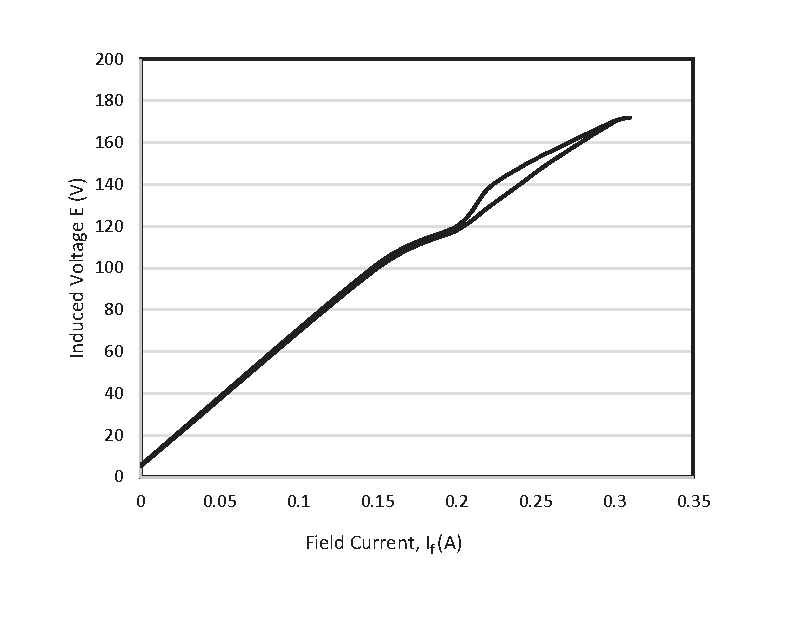
\includegraphics[width=1.2\textwidth]{Figures/Exp02/Book1.eps}}
    \vspace{0mm}
    \caption{No load magnetization curve of a separated excited DC shunt generator.}
    \label{fig:figg3}
\end{figure}
\vspace{20mm}




%**********************************************
\FloatBarrier
\section{Discussions}
The residual voltage was found 5.15 V when the current was at 0 ampere at the beginning of the experiment. The highest value of voltage was found 172 V at 0.31 ampere and the lowest voltage was found 100 V in 0.15 ampere. After turning the power on, proper distance was maintained with the wires and with the back of the circuit board. The rotation of the motor was checked properly. The current was never decreased while increasing and never increased while decreasing. The maximum value of current was found 0.31 ampere which was the saturation point of the hysteresis loop. An induction motor was used here as a prime mover and its speed was fixed at 1472 rpm during the whole experiment. All the reading in the voltmeter and the ammeter was measured as accurately as possible. While increasing the value of the rheostat, the value of the current was increased carefully so that it doesn't exceed more than 1 ampere. Otherwise the circuit can be damaged. The connection of the wires were connected properly.

\section{Conclusions}
The hysteresis loop that was plotted from the readings did not have a proper magnetic  retentivity for which a proper hysteresis loop wasn't found. Different types of errors could be the reason behind it. Not taking the accurate readings of ammeter and voltmeter, not fixing the speed of the motor accurately and the up downs of the supply voltage could be the main errors. These errors made the plotted graph different from the actual one that was supposed to be generated. But if these errors can be eliminated completely then the proper hysteresis loop could be possibly generated. 


%%%%%%%%%%%%%%% Bibliography %%%%%%%%%%%%%%%%%%
%%%%%%%%%%%%%%% Uncomment only if you need %%%%
% If you need any citations then follow this:
% An article \cite{anarticle}\\
% A book \cite{abook}\\
% A series \cite{bookseries}\\
% Someone's thesis \cite{thesis}\\
% Some technical report \cite{report}\\
% A collection \cite{collection}\\
% Visited website \cite{website}\\
% Accepted for publication \cite{acceptedpub}\\
% Submitted for publication \cite{unpub}\\
% Not published \cite{notpub}\\
% Conversation \cite{conv}
% \addcontentsline{toc}{chapter}{\bibname}
% \bibliographystyle{IEEEtran} 
% \bibliography{asmbbiblio}
%************** End of Bibliography ***********



%**********************************************
%************** End of Student's Part *********
%************** End of the Report *************
%**********************************************